\documentclass{article}
\usepackage{amsmath}
\usepackage{tikz}
\usepackage{graphicx}
\usepackage[toc,page]{appendix}
\usetikzlibrary{positioning}
\begin{document}

\title {money heist}
\author {ertosns}
\date {2023/5/5}
\maketitle

\section {leader election}
\subsection{democratized random lottery seed}
randomness $\eta_i$ in the $y$ variable in the leader election comparison, is the output of VRF.
$$\eta_i=VRF(\eta_{i-1}||slot_{id}, coin_{sk})$$  which is publicly verifiable through $verify(\eta_{i-1}||slot_{id}, coin_{pk})$, where $coin_{pk}$ is constrained as public input, and keypair $(coin_{sk},coin_{pk})$ is protected against grinding attack by published nullifier in the same contract, has advantage over ouroboros, which reduce the grinding effect through multiple queries for the random oracle for favoring high probability of winning by limiting the number of queries to the random oracle.  \cite{ouroboros_genesis}

\subsection {grinding $\eta$, and delayed stake contract}
although randomness from the lead stakeholder provider is decentralized, doesn't reveal identity of the provider, more robust than limited access global random oracle, it's deterministic, predictable, meaning, even with time-locked contracts (see \ref{timelocked}), there is a window between un-stake, and stake contracts, or for new adversarial stakeholder, it's possible to target winning at $slot_{id}$, by trying different key pairs, and picking secret key corresponding with lowest \emph{y} possible.
that attack can be prevented by delaying reward proposals from newly staked coins by N slots, N be at least 1, N being a security parameter.

\subsection {omerta attack}
although selecting key pairs corresponding of $\eta$ with lowest corresponding $y$ using public on-chain data is fixed, it's still possible to make off-chain agreements, for example at slot i if the contract execution is delayed N slots, it's possible through N agreements with winners of slots \emph{i} to \emph{i+N}, and since calculation of $\eta$ is predictable, it's possible to pick elect key pair corresponding to lowest \emph{y} at slot i+N+1 in the future, early at i slot.
note that the off-chain agreement is done with probabilistic winners, but once this attack is done once (even if possible with low probability), the adversaries will have high leverage on winning, by mining lowest possible \emph{y}.

the attack can be fixed, by introducing unpredictable random parameter: $$\eta_i = VRF(\eta_{i-1}||hash(block_{i-2})||slot_i, sk)$$


note! secret key is constrained 1 slot ahead (assume $N=1$ for simplicity), and grinding isn't possible since the staked coin is restricted from reward proposals for 1 slot, and $\eta_{i-1}$ isn't known yet, omerta attack isn't possible since $hash(block_{i-2}))$ isn't known ahead of time.

\subsection {perpetual lead with predictable block hash}



slots are divided into N+2 cycles, (N is security parameter $N \ge 1$), adversary assume winning lottery in the consecutive slots i to i+N, with certain probability, then winning leadership at slot i+N+1 becomes highly probable, only the first block at slot i include a single stake transaction (note staked DRK execution is delayed to slot i+N+1), rest of blocks i+1 to i+N are left with empty transactions, then predicting $\eta_i$ to $\eta_{i+N+1}$ is possible, and thus grinding attack can be executed.

\begin{figure}
  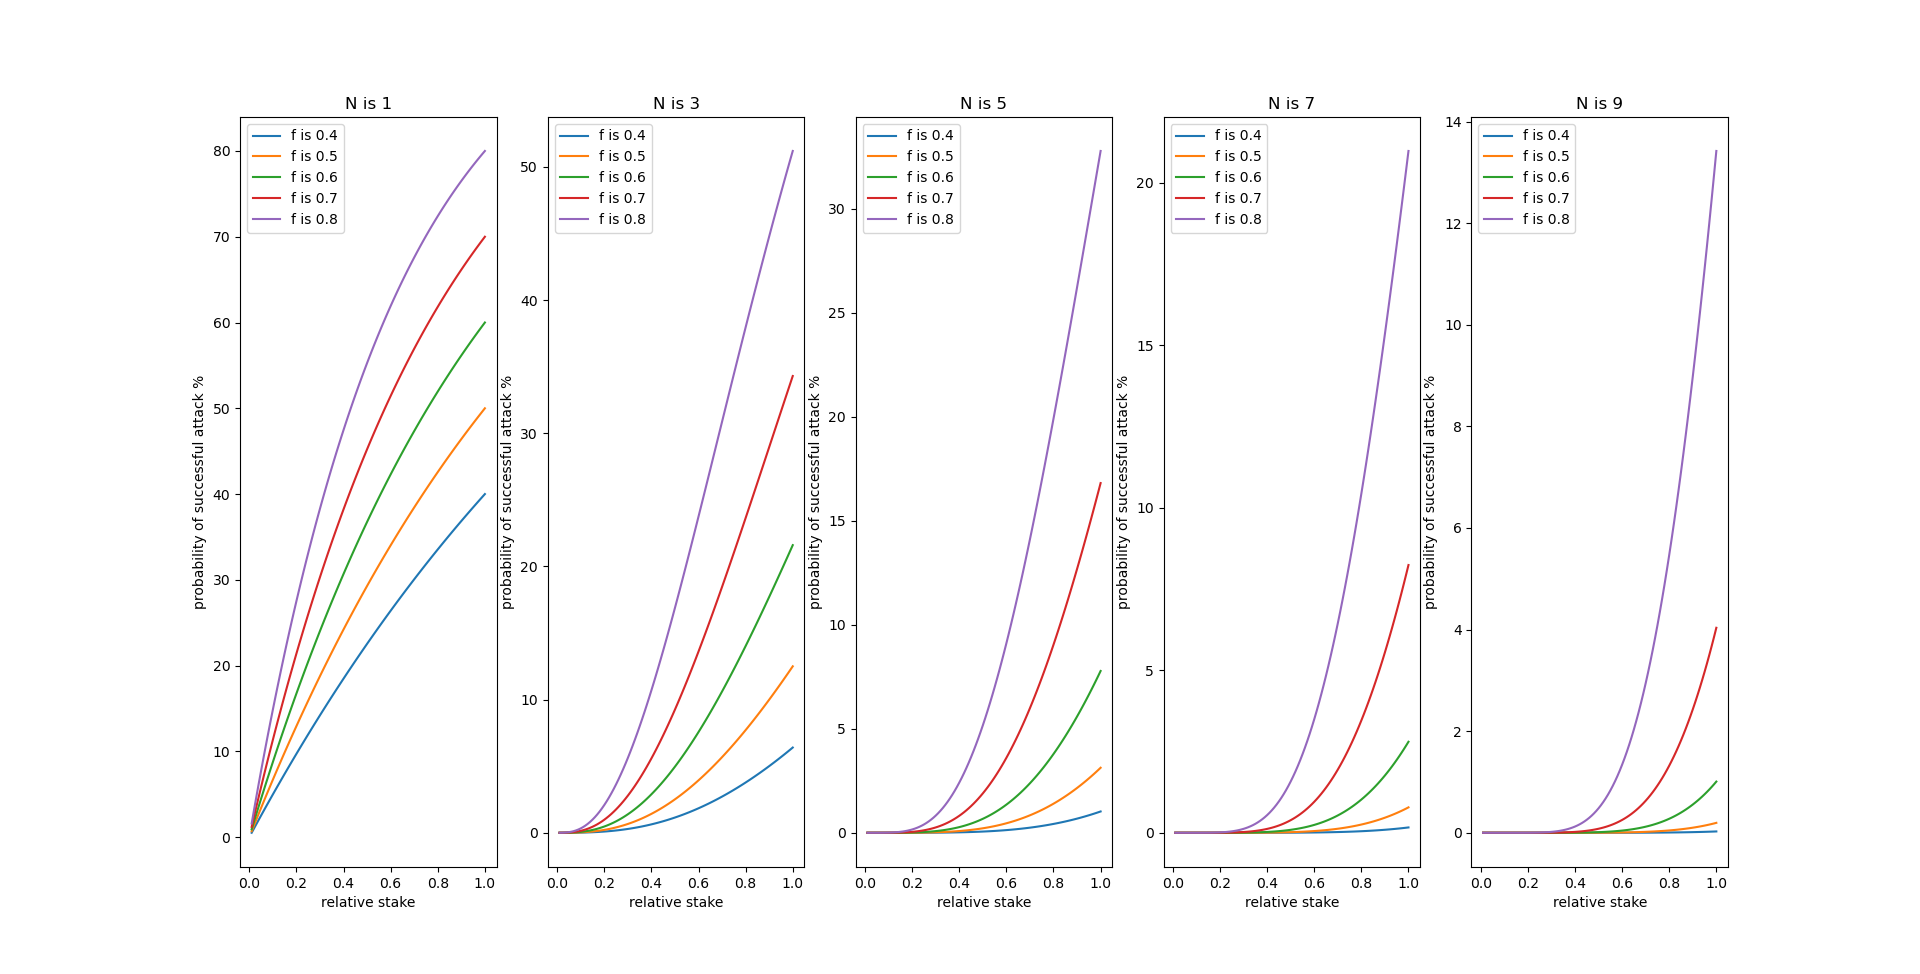
\includegraphics[width=1.2\textwidth,right]{prob.png}
  \caption{probability of attack for different security parameter}
\end{figure}


if we plot that probability of successful attack, for N (security parameter) delayed slots, function of relative stake (see figure 1), from graph we  note that even with 100% of stake,  assuming average secondary controller output f is 0.6 (simulation shows close results), then the probability of successful attack is ~ 1%, for 60% staked ratio, and f is 0.6 probability of successful attack is close to zero.

\subsection {conclusion}
the omerta attack with perpetual lead is of diminishing probability of success for security parameter $N \ge 9$.

\section{chain fork}
fork can occur when multiple stakeholders publish proposal for valid proof of leadership.
winning stakeholder can choose to fork with a new block, extend a chain, or extend chanonical longest chain.

\subsection{fork finalization}
finalization is a compound of longest chain, and single leadership frequency, at the end of any slot, finalization, and re-syncing happen when there is single leader per slot, single leader frequency is controller with secondary discrete PID controller in cascade control.
such mechanism is resilient to bribery attack \cite{attack_bribery}, and NAS attack (when the stakeholder write a transaction in one chain, and rewrite the transaction in parallel chain of equivalent stake, and equal fork depth, using relatively small stake) since probability of winning leadership with single leader frequency at small stake at more than one slot during the fork depth  is of diminishing probability.
% TODO exercise what is length of the fork to win two slots for example for someone with even 1,5,10% of stake.


\section {time frequency}
blockchain lifetime is series of epochs

\subsection {epoch}
multiple slots during which the reward value is fixed, and set by primary controller in the cascade control mechanism \cite{cascade}, and stake is dynamic different from the concept of the epoch in ouroboros, in which the epoch has frozen stake for leadership purposes.

\subsection {slot}
period of time in which new block is issued

\subsection {span}
leader election span of time, which can be unspecified period using controller, or fixed 1/3 of slot as described in khonsu \cite{khonsu} during which leaders for slots in the future are elected.

\section {timelocked contract}
\label{timelocked}
\subsection {grinding attack in stake, unstake contracts}
stakeholders can move funds between different accounts during the slot for higher probability of winning, such attack can be prevented via timelocked contracts.



\begin{thebibliography}{999}

\bibitem{ouroboros_genesis}
  Ouroboros Genesis
  \emph{Composable Proof-of-Stake Blockchains with Dynamic Availability},
  Christian Badertscher, Et al,
  22-February-2019

\bibitem{attack_bribery}
  bribery attack
  \emph{Lecture 18: Bribery and stake grinding attacks},
  David Tse,
  Stanford University, Spring 2020
  04-June-2020

\bibitem{cascade}
  cascade,
  \emph{consensus high incentive monetary policy},
  ertosns,
  15-4-2023

\bibitem{khonsu}
  khonsu,
  \emph{darkfi khonsu consensus},
  ertosns,
  31-12-2022


\end{thebibliography}


\end{document}
